%\documentclass[12pt]{article}
%
%\usepackage{fancyhdr} % Required for custom headers
%\usepackage{lastpage} % Required to determine the last page for the footer
%\usepackage{extramarks} % Required for headers and footers
%\usepackage[usenames,dvipsnames]{color} % Required for custom colors
%\usepackage{graphicx} % Required to insert images
%\usepackage{listings} % Required for insertion of code
%\usepackage{courier} % Required for the courier font
%\usepackage{lipsum} % Used for inserting dummy 'Lorem ipsum' text into the template
%\usepackage{amsmath}
%\usepackage{caption}
%\usepackage{multirow}
%\usepackage{graphicx}
%\usepackage{amssymb}
%\usepackage{caption}
%\usepackage{graphicx}
%\usepackage{subcaption}
%\usepackage{algorithm}
%\usepackage{algpseudocode}
%\usepackage[dvipsnames]{xcolor}
%
%\newcommand*{\addheight}[2][.5ex]{%
%	\raisebox{0pt}[\dimexpr\height+(#1)\relax]{#2}%
%}
%% Margins
%\topmargin=-0.45in
%\evensidemargin=0in
%\oddsidemargin=0in
%\textwidth=6.5in
%\textheight=9.0in
%\headsep=0.25in
%\headheight=15.0pt
%
%
%\linespread{1.1} % Line spacing
%
%% Set up the header and footer
%\pagestyle{fancy}
%\lhead{\hmwkAuthorName} % Top left header
%\chead{\hmwkClassHeader: \hmwkTitle} % Top center head
%\cfoot{} % Bottom center footer
%\rfoot{Page\ \thepage\ of\ \protect\pageref{LastPage}} % Bottom right footer
%\renewcommand\headrulewidth{0.4pt} % Size of the header rule
%\renewcommand\footrulewidth{0.4pt} % Size of the footer rule
%
%\setlength\parindent{0pt} % Removes all indentation from paragraphs
%
%%----------------------------------------------------------------------------------------
%%	DOCUMENT STRUCTURE COMMANDS
%%	Skip this unless you know what you're doing
%%----------------------------------------------------------------------------------------
%
%% Header and footer for when a page split occurs within a problem environment
%\newcommand{\enterProblemHeader}[1]{
%	\nobreak\extramarks{#1}{#1 continued on next page\ldots}\nobreak
%	\nobreak\extramarks{#1 (continued)}{#1 continued on next page\ldots}\nobreak
%}
%
%% Header and footer for when a page split occurs between problem environments
%\newcommand{\exitProblemHeader}[1]{
%	\nobreak\extramarks{#1 (continued)}{#1 continued on next page\ldots}\nobreak
%	\nobreak\extramarks{#1}{}\nobreak
%}
%
%\setcounter{secnumdepth}{0} % Removes default section numbers
%\newcounter{homeworkProblemCounter} % Creates a counter to keep track of the number of problems
%
%\newcommand{\homeworkProblemName}{}
%\newenvironment{homeworkProblem}[1][Problem \arabic{homeworkProblemCounter}]{ % Makes a new environment called homeworkProblem which takes 1 argument (custom name) but the default is "Problem #"
%	\stepcounter{homeworkProblemCounter} % Increase counter for number of problems
%	\renewcommand{\homeworkProblemName}{#1} % Assign \homeworkProblemName the name of the problem
%	\section{\homeworkProblemName} % Make a section in the document with the custom problem count
%	\enterProblemHeader{\homeworkProblemName} % Header and footer within the environment
%}{
%	\exitProblemHeader{\homeworkProblemName} % Header and footer after the environment
%}
%
%\newcommand{\problemAnswer}[1]{ % Defines the problem answer command with the content as the only argument
%	\noindent\framebox[\columnwidth][c]{\begin{minipage}{0.98\columnwidth}#1\end{minipage}} % Makes the box around the problem answer and puts the content inside
%}
%
%\newcommand{\homeworkSectionName}{}
%\newenvironment{homeworkSection}[1]{ % New environment for sections within homework problems, takes 1 argument - the name of the section
%	\renewcommand{\homeworkSectionName}{#1} % Assign \homeworkSectionName to the name of the section from the environment argument
%	\subsection{\homeworkSectionName} % Make a subsection with the custom name of the subsection
%	\enterProblemHeader{\homeworkProblemName\ [\homeworkSectionName]} % Header and footer within the environment
%}{
%	\enterProblemHeader{\homeworkProblemName} % Header and footer after the environment
%}
%
%%----------------------------------------------------------------------------------------
%%	NAME AND CLASS SECTION
%%----------------------------------------------------------------------------------------
%
%\newcommand{\hmwkTitle}{Assignment\ \#2} % Assignment title
%\newcommand{\hmwkClass}{Machine Learning} % Course/class
%\newcommand{\hmwkClassHeader}{Machine Learning} % Course/class
%\newcommand{\hmwkAuthorName}{Shikhar Vashishth} % Your name
%\newcommand{\hmwkAuthorID}{M.Tech CSA - 13374} % Your ID
%
%%----------------------------------------------------------------------------------------
%%	TITLE PAGE
%%----------------------------------------------------------------------------------------
%
%\title{
%	\vspace{2in}
%	\textmd{\textbf{\hmwkClass}}\\ 
%	\textmd{\textbf{\hmwkTitle}}\\
%	\vspace{3in}
%}
%
%\author{\textbf{\hmwkAuthorName} \\ {\small \hmwkAuthorID}}
%\date{} % Insert date here if you want it to appear below your name
%
%%----------------------------------------------------------------------------------------
%
%\begin{document}
%	
%\maketitle
%\newpage
%	
%	
%\clearpage
%%************************************PROBLEM 1********************************************
%\begin{homeworkProblem}
%\subsection{Part (a):}
%
%
%\textit{NOTE: I have used cvpartition method for creating cross-validation set, so my results may not match with the standard solution key.}
%
%\begin{figure}[h]
%	\centering
%	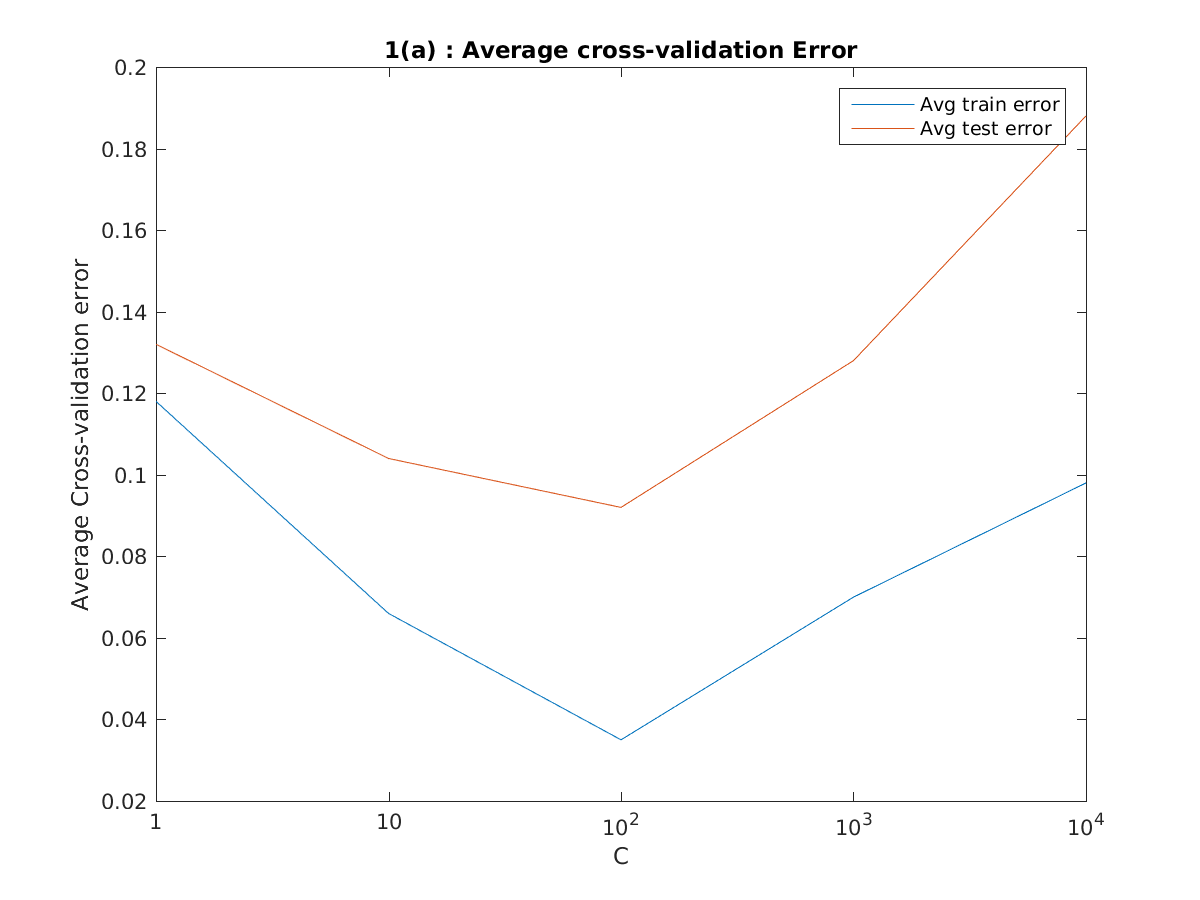
\includegraphics[width=16cm]{../hw2-code-data/hw2-code-data/Problem1/plot/1a}
%\end{figure}
%
%
%\begin{center}
%	\begin{tabular}{||c c c||} 
%		\hline
%		C & Avg Training Error & Avg Test Error \\ [0.5ex] 
%		\hline\hline
%		1 & 0.1180 & 0.1320  \\ \hline
%		10 & 0.0660 & 0.1040  \\ \hline
%		\textbf{100} & \textbf{0.0350} & \textbf{0.0920}  \\ \hline
%		1000 & 0.0700 & 0.1280  \\ \hline
%		10000 & 0.0980 & 0.1880  \\ \hline
%		\hline
%	\end{tabular}
%\end{center}
%
%We can see from the above results that the best performance is obtained at $C = 100$. 
%\newpage
%
%%***************************************PART 1(b)*************************************
%\subsection{Part (b):}
%
%\subsubsection{Using Linear kernel}
%
%\begin{figure}[h]
%	\centering
%	\begin{subfigure}[b]{0.45\textwidth}
%		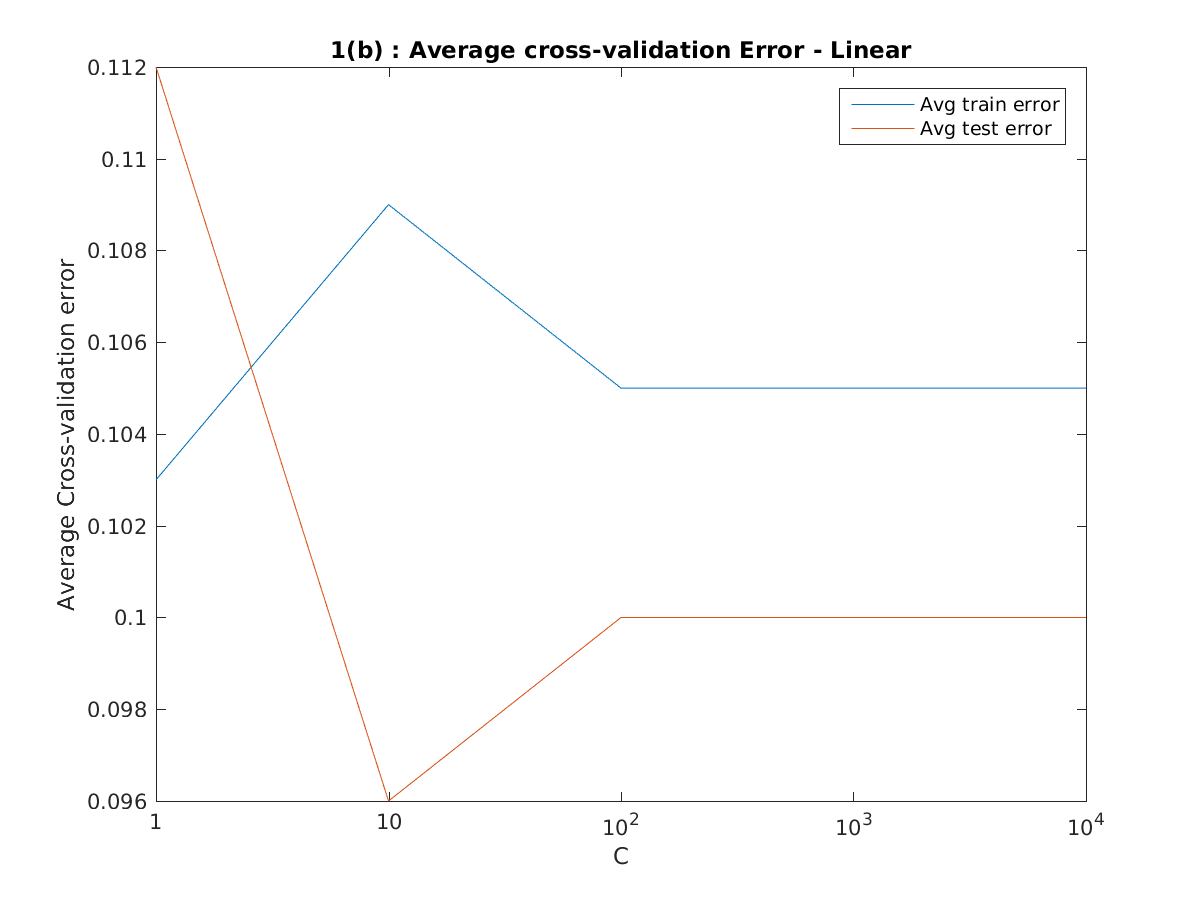
\includegraphics[width=\textwidth]{../hw2-code-data/hw2-code-data/Problem1/plot/1b_linear}
%		\caption{5-fold cross validation error using linear kernel}
%	\end{subfigure}
%	\hfill
%	\begin{subfigure}[b]{0.5\textwidth}
%		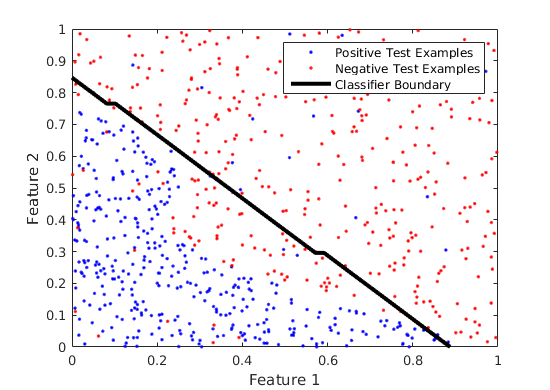
\includegraphics[width=\textwidth]{../hw2-code-data/hw2-code-data/Problem1/plot/1b_linear_best}
%		\caption{Performance of linear kernel with C = 10}
%	\end{subfigure}
%\end{figure}
%
%\begin{table}[h]
%	\begin{center}
%		\begin{tabular}{||c c c||} 
%			\hline
%			C & Avg Training Error & Avg Test Error \\ [0.5ex] 
%			\hline\hline
%			1 & 0.1030 & 0.1120  \\ \hline
%			\textbf{10} & \textbf{0.1090} & \textbf{0.0960}  \\ \hline
%			100 & 0.1050 & 0.1000  \\ \hline
%			1000 & 0.1050 & 0.1000  \\ \hline
%			10000 & 0.1050 & 0.1000  \\ \hline
%			\hline
%		\end{tabular}
%	\end{center}
%\end{table}
%
%
%Best C: \textbf{10} \\
%Training error on full dataset: \textbf{0.1040}\\
%Test error on full dataset: \textbf{0.1320}
%
%
%
%\newpage
%
%\subsubsection{Using degree 2 Polynomial kernel}
%
%\begin{figure}[h]
%	\centering
%	\begin{subfigure}[b]{0.45\textwidth}
%		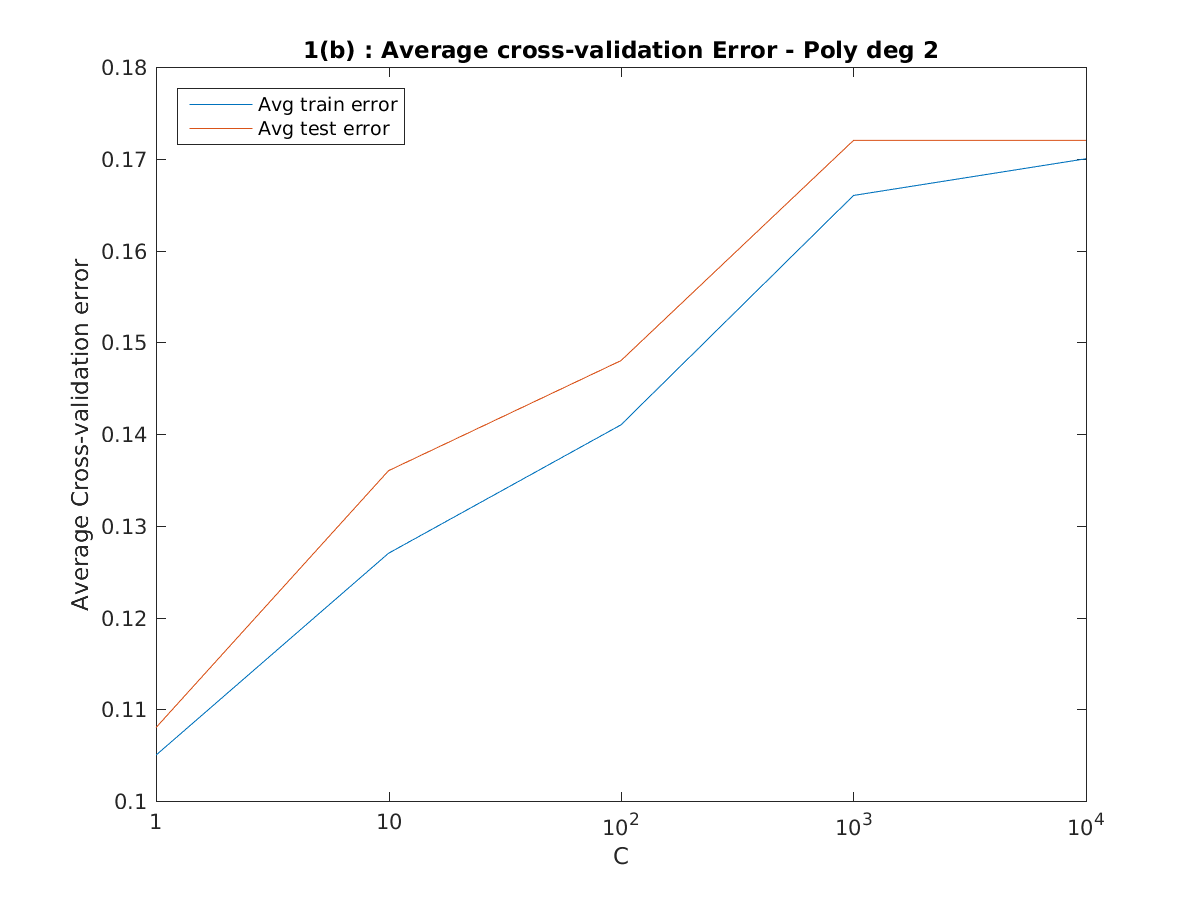
\includegraphics[width=\textwidth]{../hw2-code-data/hw2-code-data/Problem1/plot/1b_pdeg2}
%		\caption{5-fold cross validation error using degree 2 polynomial}
%	\end{subfigure}
%	\hfill
%	\begin{subfigure}[b]{0.5\textwidth}
%		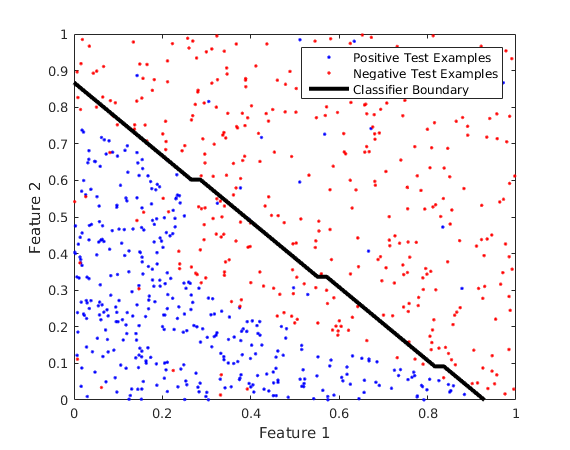
\includegraphics[width=\textwidth]{../hw2-code-data/hw2-code-data/Problem1/plot/1b_pdeg2_best}
%		\caption{Performance with polynomial degree 2  kernel with C = 1}
%	\end{subfigure}
%\end{figure}
%
%\begin{table}[h]
%	\begin{center}
%		\begin{tabular}{||c c c||}
%			\hline
%			C & Avg Training Error & Avg Test Error \\ [0.5ex] 
%			\hline\hline
%			\textbf{1} & \textbf{0.1050} & \textbf{0.1080}  \\ \hline
%			10 & 0.1270 & 0.1360  \\ \hline
%			100 & 0.1410 & 0.1480  \\ \hline
%			1000 & 0.1660 & 0.1720  \\ \hline
%			10000 & 0.1700 & 0.1720  \\ \hline
%			\hline
%		\end{tabular}
%	\end{center}
%\end{table}
%Best C: \textbf{1} \\
%Training error on full dataset: \textbf{0.1080}\\
%Test error on full dataset: \textbf{0.1360}
%
%
%\pagebreak
%
%\subsubsection{Using Polynomial degree 3 Kernel}
%
%
%\begin{figure}[h]
%	\centering
%	\begin{subfigure}[b]{0.45\textwidth}
%		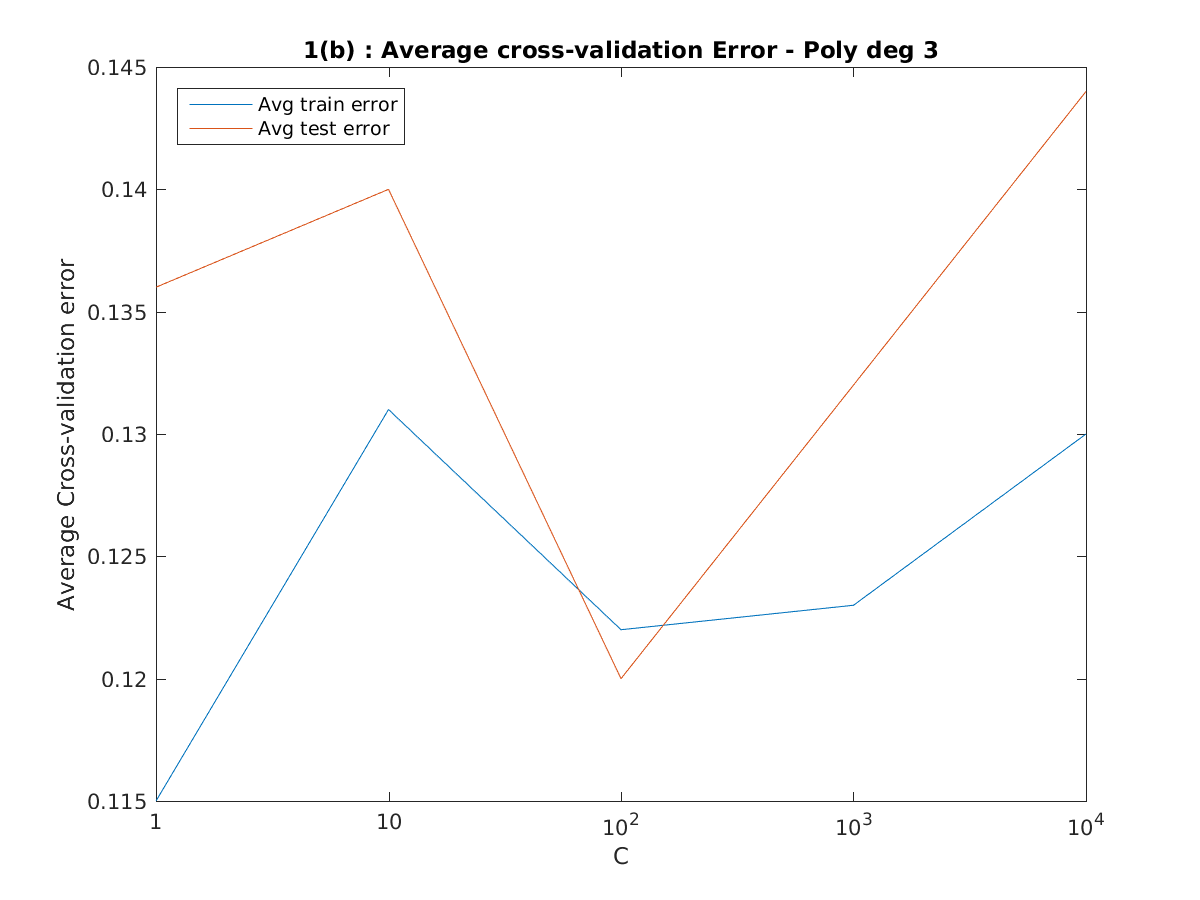
\includegraphics[width=\textwidth]{../hw2-code-data/hw2-code-data/Problem1/plot/1b_pdeg3}
%		\caption{Cross validation error using degree 3 polynomial kernel}
%	\end{subfigure}
%	\hfill
%	\begin{subfigure}[b]{0.5\textwidth}
%		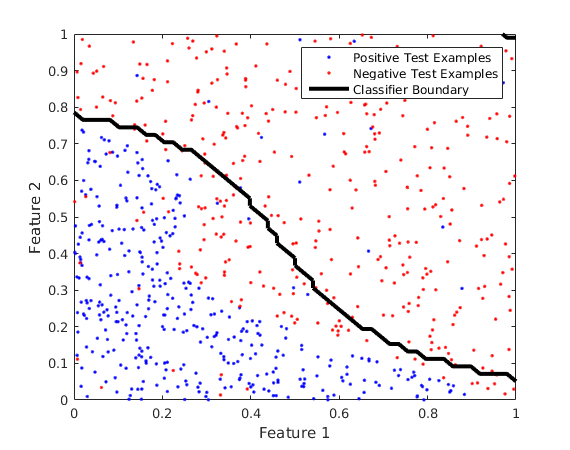
\includegraphics[width=\textwidth]{../hw2-code-data/hw2-code-data/Problem1/plot/1b_pdeg3_best}
%		\caption{Performance with polynomial degree 3 kernel with C = 100}
%	\end{subfigure}
%\end{figure}
%
%\begin{table}[h]
%	\begin{center}
%		\begin{tabular}{||c c c||} 
%			\hline
%			C & Avg Training Error & Avg Test Error \\ [0.5ex] 
%			\hline\hline
%			1 & 0.1150 & 0.1360  \\ \hline
%			10 & 0.1310 & 0.1400  \\ \hline
%			\textbf{100} & \textbf{0.1220} & \textbf{0.1200}  \\ \hline
%			1000 & 0.1230 & 0.1320  \\ \hline
%			10000 & 0.1300 & 0.1440  \\ \hline
%			\hline
%		\end{tabular}
%	\end{center}
%\end{table}
%
%Best C: \textbf{100} \\
%Training error on full dataset: \textbf{0.1080}\\
%Test error on full dataset: \textbf{0.1440}
%
%\newpage
%
%\subsubsection{Using RBF Kernel}
%
%\begin{figure}[h]
%	\centering
%	\begin{subfigure}[b]{0.45\textwidth}
%		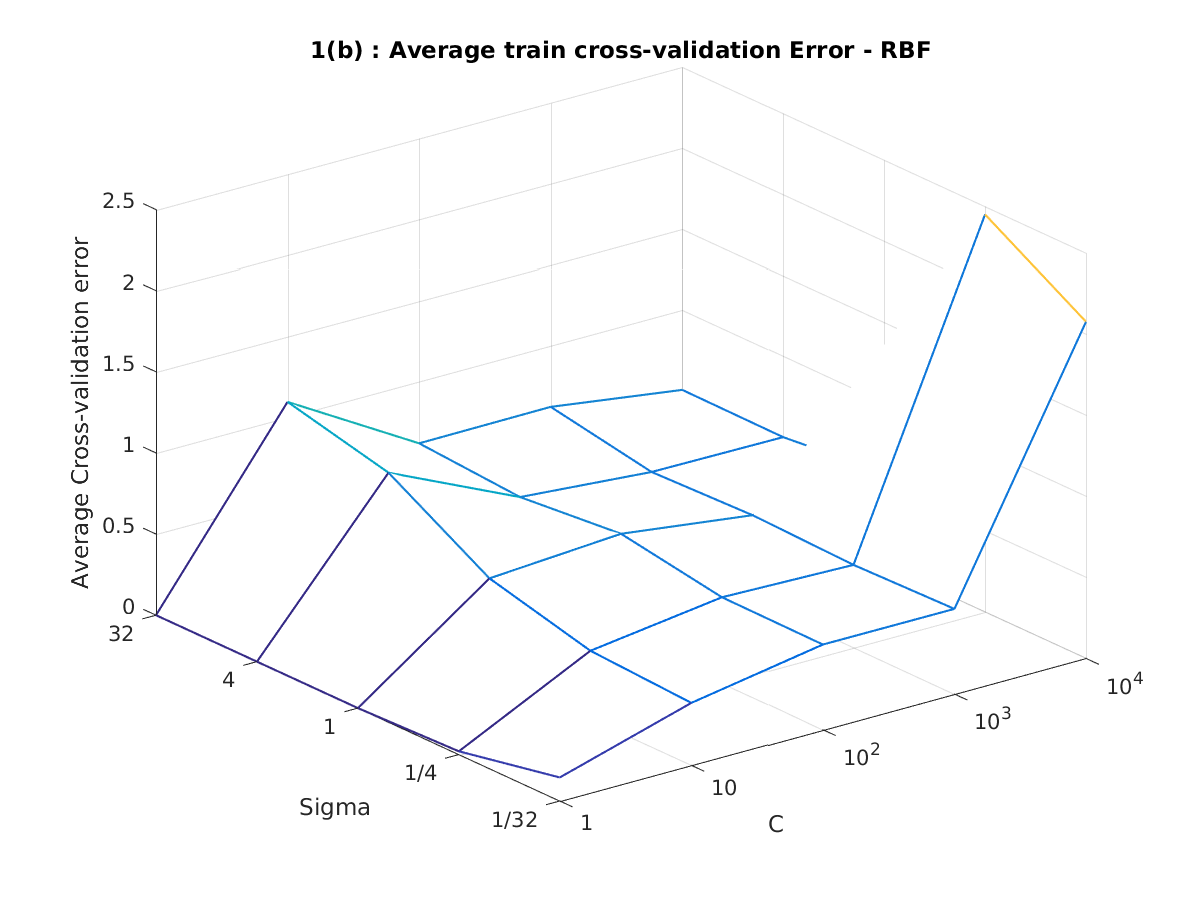
\includegraphics[width=\textwidth]{../hw2-code-data/hw2-code-data/Problem1/plot/1b_rbf_train}
%		\caption{Cross validation error on training data using RBF kernel}
%	\end{subfigure}
%	\hfill
%	\begin{subfigure}[b]{0.5\textwidth}
%		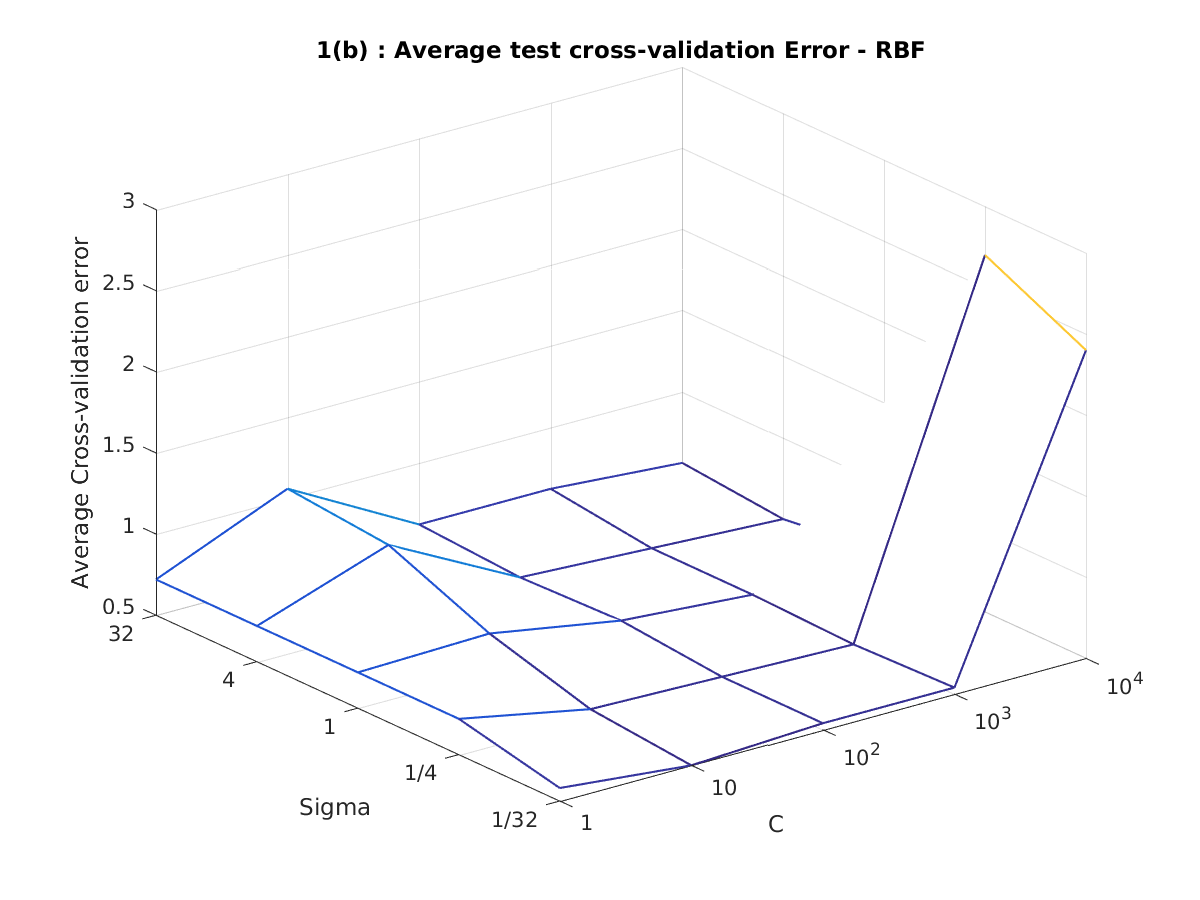
\includegraphics[width=\textwidth]{../hw2-code-data/hw2-code-data/Problem1/plot/1b_rbf_test}
%		\caption{cross validation error on test data using RBF kernel}
%	\end{subfigure}
%\end{figure}
%
%\textbf{Training Error:}
%\begin{center}
%	\begin{tabular}{||c || c c c c c||} 
%		\hline
%		C/sigma & 1/32 &  1/4 &  1 & 4 & 32 \\ [0.5ex] 
%		\hline\hline
%		1 & 0.1550   & 0.4150   & 0.5300   & 0.5250   & 2.0600 \\ \hline
%		10 & 0.0200   & 0.3950   & 0.5300   & 0.5150   & 2.4500 \\ \hline
%		100 & 0   & 0.6750   & 0.6300   & 0.5150   & 0.5750 \\ \hline
%		1000 & 0   & 0.8700   & 0.5700   & 0.5250   & 0.5300 \\ \hline
%		10000 & 0   & 0.8650   & 0.6350   & 0.6150   & 0.5350 \\ \hline
%		\hline
%	\end{tabular}
%\end{center}
%	
%\textbf{Test Error:}
%\begin{center}
%	\begin{tabular}{||c || c c c c c||} 
%		\hline
%		C/sigma & 1/32 & \textbf{ 1/4} &  1 & 4 & 32 \\ [0.5ex] 
%		\hline\hline
%		1 & 0.6400  &  0.5400  &  0.5800   & 0.6600   & 2.2800 \\ \hline
%		\textbf{10} & 0.7400  &  \textbf{0.4800}  &  0.5800   & 0.5600   & 2.7000 \\ \hline
%		100 & 0.7600  &  0.6200  &  0.6200   & 0.5400   & 0.5800 \\ \hline
%		1000 & 0.7600  &  0.7800  &  0.6000   & 0.5800   & 0.6000 \\ \hline
%		10000 & 0.7600  &  0.8600  &  0.6600   & 0.6400   & 0.5000 \\ \hline
%		\hline
%	\end{tabular}
%\end{center}
%
%Best C: \textbf{10} \\
%Best Sigms: \textbf{1/4} \\
%Training error: \textbf{0.0880}\\
%Test error: \textbf{0.1387}
%
%
%\begin{figure}[h]
%	\centering
%	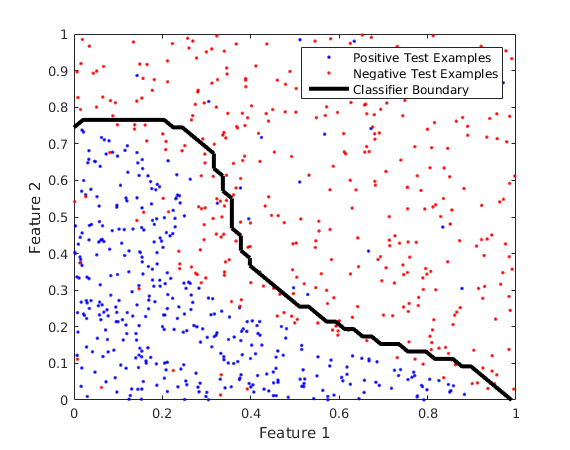
\includegraphics[width=16cm]{../hw2-code-data/hw2-code-data/Problem1/plot/1b_rbf_best}
%	\caption{Performance with RBF kernel with C = 10 and sigma = 1/4}
%\end{figure}
%
%\newpage
%\subsection{Part (c):}
%Error on the test set in case of SVM is \textbf{0.1168}, whereas in the case of logistic regression error is \textbf{0.1191}. We can clearly see that the performance of SVM is better than performance of logistic regression. The performance of SVM is better, because it fits a maximal margin linear classifier which gives us better generalization any than other linear classifiers.
%\end{homeworkProblem}
%
%%************************************PROBLEM 2**************************************
%\begin{homeworkProblem}
%\subsection{Part (c):}
%Training Error: \textbf{101.3872} \\
%Testing Error: \textbf{26.8586}
%
%\newpage
%\subsection{Part (d):}
%\subsubsection{Error on Training folds:}
%\begin{table}[h]
%	\begin{center}
%		\begin{tabular}{||c||c c c c c||} 
%			\hline
%			$\lambda$/Folds & Fold 1 &  Fold 2 &  Fold 3 & Fold 4 & Fold 5 \\ [0.5ex] 
%			\hline\hline
%			0.01  & 105.3216 &  98.2991 & 100.0530 & 101.8518 & 101.2350 \\ \hline
%			0.1  & 105.3216 &  98.2991 & 100.0530 & 101.8518 & 101.2350 \\ \hline
%			1  & 105.3245 &  98.3021 & 100.0561 & 101.8551 & 101.2378 \\ \hline
%			10  & 105.5627 &  98.5515 & 100.3096 & 102.1285 & 101.4685 \\ \hline
%			100  & 112.5263 & 105.6139 & 107.3352 & 109.6258 & 108.1266 \\ \hline
%			\hline
%		\end{tabular}
%	\end{center}
%\end{table}
%
%
%
%\subsubsection{Error on test folds}
%\begin{table}[h]
%	\begin{center}
%		\begin{tabular}{||c || c c c c c ||} 
%			\hline
%			$\lambda$/Folds & Fold 1 &  Fold 2 &  Fold 3 & Fold 4 & Fold 5 \\ [0.5ex] 
%			\hline\hline
%			0.01 & 85.7615 & 113.9051 & 106.7523 &  99.7846 & 102.3173 \\ \hline
%			0.1 & 85.7628 & 113.9046 & 106.7523 &  99.7746 & 102.3238 \\ \hline
%			1 & 85.7780 & 113.9033 & 106.7560 &  99.6801 & 102.3902 \\ \hline
%			10 & 86.0910 & 114.1163 & 107.0459 &  99.1158 & 103.1771 \\ \hline
%			100 & 92.4212 & 121.1080 & 115.0829 & 103.6544 & 112.0226 \\ \hline
%			\hline
%		\end{tabular}
%	\end{center}
%\end{table}
%
%\subsubsection{Average cross-validation training and test error}
%\begin{table}[h]
%	\begin{center}
%		\begin{tabular}{||c c c||} 
%			\hline
%			C & Training Error & Test Error \\ [0.5ex] 
%			\hline\hline
%			0.01 & 101.3521 & 101.7041 \\ \hline
%			0.1 & 101.3521 & 101.7036 \\ \hline
%			\textbf{1} & \textbf{101.3551} & \textbf{101.7015} \\ \hline
%			10 & 101.6042 & 101.9092 \\ \hline
%			100 & 108.6456 & 108.8578 \\ \hline
%			\hline
%		\end{tabular}
%	\end{center}
%\end{table}
%
%\paragraph{Cross-Validation results}
%The average error for first four $\lambda$ values ($.01, 0.1, 1, 10$) are almost the same but we can see from the above table (test error) that with $\lambda = 1$ the test error is slightly lesser than with other $\lambda$ values.
% 
%\begin{figure}[h]
%	\centering
%	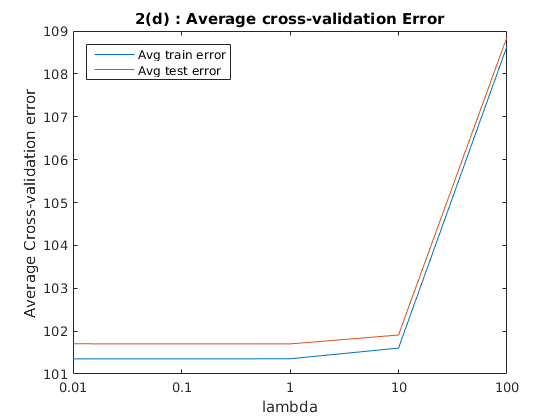
\includegraphics[width=9.5cm]{../hw2-code-data/hw2-code-data/Problem2/plot/2d_avg_error}
%\end{figure}
%
%\newpage
%  \begin{table}[h]
%	\begin{center}
%		\begin{tabular}{||c c c||} 
%			\hline
%			C & Training Error & Test Error \\ [0.5ex] 
%			\hline\hline
%			0.01 & 101.3872 & 26.8575 \\ \hline
%			0.1 & 101.3872 & 26.8476 \\ \hline
%			1 & 101.3891 & 26.7510 \\ \hline
%			\textbf{10} & \textbf{101.5543} & \textbf{26.0140} \\ \hline
%			100 & 107.1628 & 26.8059 \\ \hline
%			\hline
%		\end{tabular}
%		\caption{Training and test error with complete data set}
%	\end{center}
%\end{table}
%\paragraph{Results with complete data sets}
%We can see from the above results that the best test error is obtained with $\lambda = 10$ which doesn't match with the lambda value obtained from the cross-validation method.
%
%\paragraph{Comparison with linear least square regression}
%Although, as compared to linear least squares the training set error has slightly increased in the case of ridge regression, but the test error has reduced from \textbf{26.8586 to 26.0140}, which shows that ridge regression gave us a more generalized classifier.
%
%\newpage
%\subsection{Part (f):}
%\subsubsection{Error on training folds}
%\begin{center}
%	\begin{tabular}{||c||c c c c c||} 
%		\hline
%		$\lambda$/Folds & Fold 1 &  Fold 2 &  Fold 3 & Fold 4 & Fold 5 \\ [0.5ex] 
%		\hline\hline
%		0.01 & 68.1371  & 62.3615  & 86.5153  & 67.1764  & 67.4253 \\ \hline
%		0.1 & 68.0578  & 62.2227  & 63.6664  & 66.0992  & 65.0810 \\ \hline
%		1 & 68.0666  & 62.2314  & 63.6733  & 66.1081  & 65.0863 \\ \hline
%		10 & 68.5379  & 62.7093  & 64.0655  & 66.5871  & 65.4939 \\ \hline
%		100 & 73.0739  & 67.1732  & 68.1676  & 71.1525  & 70.1366 \\ \hline
%		\hline
%	\end{tabular}
%\end{center}
%
%\subsubsection{Error on test folds}
%\begin{center}
%	\begin{tabular}{||c||c c c c c||} 
%		\hline
%		$\lambda$/Folds & Fold 1 &  Fold 2 &  Fold 3 & Fold 4 & Fold 5 \\ [0.5ex] 
%		\hline\hline
%		0.01 & 53.4618 &  76.8461  & 95.0592  & 61.7699  & 68.0263 \\ \hline
%		0.1 & 53.3219 &  76.6653  & 71.0157  & 61.0810  & 65.4354 \\ \hline
%		1 & 53.2795 &  76.6249  & 71.1206  & 61.0230  & 65.4367 \\ \hline
%		10 & 53.4503 &  76.9216  & 72.2954  & 61.1128  & 65.7226 \\ \hline
%		100 & 57.5729 &  82.2489  & 78.7476  & 65.3079  & 68.1862 \\ \hline
%		\hline
%	\end{tabular}
%\end{center}
%
%\subsubsection{Average cross-validation training and test error}
%
%\begin{center}
%	\begin{tabular}{||c c c||} 
%		\hline
%		C & Training Error & Test Error \\ [0.5ex] 
%		\hline\hline
%		0.01 & 70.3231 & 71.0327 \\ \hline
%		0.1 & 65.0254 & 65.5039 \\ \hline
%		\textbf{1} & \textbf{65.0332} &\textbf{ 65.4969} \\ \hline
%		10 & 65.4787 & 65.9005 \\ \hline
%		100 & 69.9408 & 70.4127 \\ \hline
%		\hline
%	\end{tabular}
%\end{center}
%
%
%
%\begin{figure}[h]
%	\centering
%	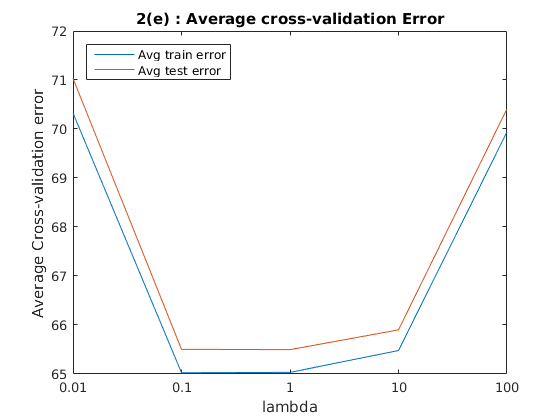
\includegraphics[width=8.5cm]{../hw2-code-data/hw2-code-data/Problem2/plot/2e_avg_error}
%\end{figure}
%
%
%\newpage
%\paragraph{Cross Validation results}
%We can see from the results that $\lambda = 1$ looks like the best choice for the given setting. Although, $\lambda = 0.1$ is also quite close in performance to 1 but on average results with $\lambda = 1$ are better. 
%\begin{table}[h]
%	\begin{center}
%		\begin{tabular}{||c c c||} 
%			\hline
%			C & Training Error & Test Error \\ [0.5ex] 
%			\hline\hline
%			0.01 & 66.9187 & 23.7157  \\ \hline
%			0.1 & 65.0736 & 16.0687  \\ \hline
%			1 & 65.0775 & 16.0159  \\ \hline
%			10 & 65.3960 & 14.5744  \\ \hline
%			\textbf{100} & \textbf{69.2362} & \textbf{12.8448}  \\ \hline
%			\hline
%		\end{tabular}
%		\caption{Training and test error with complete data set}
%	\end{center}
%\end{table}
%
%
%\paragraph{Results with complete data sets}
%We can see from the graph that the best test error with full data set is obtained with $\lambda = 100$ which doesn't match with the results which we obtained from the cross-validation method.
%
%\paragraph{Comparison with linear ridge regression}
%As compared to the linear ridge regression the performance in this case is much better. Both training error and test errors have reduced which shows that the actual distribution of the data can be better modelled using a polynomial of degree 3 rather than a linear model.
%\end{homeworkProblem}
%
%%*******************************PROBLEM 3*********************************************
%\newpage
%\begin{homeworkProblem}
%
%\subsection{Part (b):}
%
%\subsection{Cross-Validation}
%\subsubsection{Error on training folds}
%\begin{center}
%	\begin{tabular}{||c||c c c c c||} 
%		\hline
%		C/Folds & Fold 1 &  Fold 2 &  Fold 3 & Fold 4 & Fold 5 \\ [0.5ex] 
%		\hline\hline
%		0.01 & 113.9167 & 106.8238  & 123.0163 & 111.0709 & 114.9589 \\ \hline
%		1    & 118.7971 & 120.3559  & 113.3968 & 134.9623 & 369.5602 \\ \hline
%		100  & 106.9600 & 157.2253  & 101.7997 & 103.9910 & 438.7858 \\ \hline
%		\hline
%	\end{tabular}
%\end{center}
%
%\subsubsection{Error on test folds}
%
%\begin{center}
%	\begin{tabular}{||c||c c c c c||} 
%		\hline
%		C/Folds & Fold 1 &  Fold 2 &  Fold 3 & Fold 4 & Fold 5 \\ [0.5ex] 
%		\hline\hline
%		0.01 & 93.1396 &  125.8512 & 129.2377 & 104.1163 & 113.9241 \\ \hline
%		1    & 94.8845 &  128.5385 & 122.5024 & 128.4787 & 399.5460 \\ \hline
%		100  & 87.6967 &  160.2333 & 109.3543 & 100.2524 & 472.3654 \\ \hline
%		\hline
%	\end{tabular}
%\end{center}
%
%\begin{figure}[h]
%	\centering
%	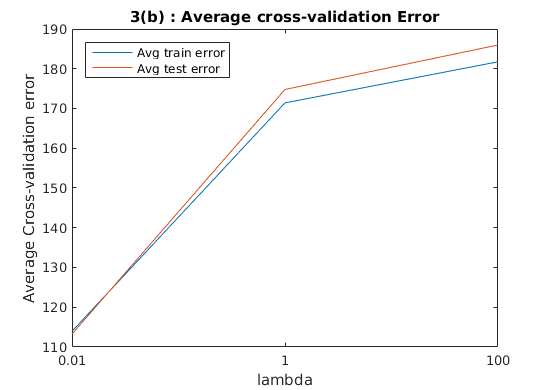
\includegraphics[width=8.5cm]{../hw2-code-data/hw2-code-data/Problem3/plot/3b}
%\end{figure}
%
%\subsubsection{Average cross-validation training and test error}
%
%\begin{center}
%	\begin{tabular}{||c c c||} 
%		\hline
%		C & Training Error & Test Error \\ [0.5ex] 
%		\hline\hline
%		\textbf{0.01} &\textbf{ 113.9573 }& \textbf{113.2538} \\ \hline
%		1    & 171.4144 & 174.7900 \\ \hline
%		100  & 181.7524 & 185.9804 \\ \hline
%		\hline
%	\end{tabular}
%\end{center}
%
%
%\paragraph{Cross Validation results}
%Cross-Validation method tells us that the best value of $C$ is 0.01, because with this value, we are getting the least average test and training error.
%
%\newpage
%\subsubsection{Training and test error on full training and test set (*1.0e+03)}
%           
%\begin{table}[h]
%	\begin{center}
%		\begin{tabular}{||c c c||} 
%			\hline
%			C & Training Error & Test Error \\ [0.5ex] 
%			\hline\hline
%			0.01 & 107.7798 & 20.6209 \\ \hline
%			\textbf{1}    & \textbf{104.8866} & \textbf{21.2221} \\ \hline
%			100  & 104.1523 & 21.5284 \\ \hline
%			\hline
%		\end{tabular}
%	\end{center}
%\end{table}
%
%\paragraph{Results with complete data sets}
%From the above results we can see that the best value of $C$ is 1, because it is giving us least test error. Hence, in this age cross-validation didn't give us the right estimate of $C$.
%
%\paragraph{Comparing with linear least squares and linear ridge regression}
%We can see from the results on entire training and test set that the performance of support vector regression is better compared to linear least squares and linear ridge regression algorithms.
%
%% *************************************************PROBLEM 3 part(c)*************************************************************
%\newpage
%\subsection{Part (c):}
%\subsection{Cross-Validation}
%\subsubsection{Error on training folds}
%\begin{center}
%	\begin{tabular}{||c||c c c c c||} 
%		\hline
%		C/Folds & Fold 1 &  Fold 2 &  Fold 3 & Fold 4 & Fold 5 \\ [0.5ex] 
%		\hline\hline
%		0.01 & 94.5786  & 83.2528  & 86.0032 &  91.7747  & 92.2636 \\ \hline
%		1    & 87.8022  & 76.3866  & 81.9559 &  85.6317  & 79.7258 \\ \hline
%		100  & 97.4177  & 80.1165  & 86.5986 &  80.7769  & 83.6444 \\ \hline
%		\hline
%	\end{tabular}
%\end{center}
%
%
%\subsubsection{Error on test folds}
%\begin{center}
%	\begin{tabular}{||c||c c c c c||} 
%		\hline
%		C/Folds & Fold 1 &  Fold 2 &  Fold 3 & Fold 4 & Fold 5 \\ [0.5ex] 
%		\hline\hline
%		0.01 & 74.4860 & 101.4484  & 97.0814  & 84.9846  & 89.8629 \\ \hline
%		1    & 68.4400 &  93.0966  & 91.9062  & 77.4420  & 79.7727 \\ \hline
%		100  & 77.2873 &  98.2538  & 97.0021  & 73.8498  & 83.1568 \\ \hline
%		\hline
%	\end{tabular}
%\end{center}
%
%\begin{figure}[h]
%	\centering
%	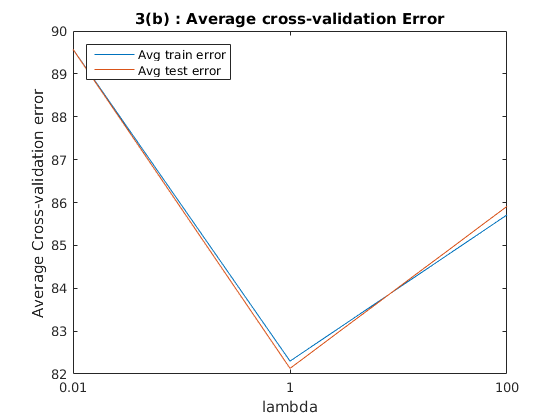
\includegraphics[width=8.5cm]{../hw2-code-data/hw2-code-data/Problem3/plot/3c}
%\end{figure}
%
%\subsubsection{Average cross-validation training and test error}
%\begin{center}
%	\begin{tabular}{||c c c||} 
%		\hline
%		C & Training Error & Test Error \\ [0.5ex] 
%		\hline\hline
%		0.01 & 89.5746 & 89.5727 \\ \hline
%		\textbf{1}    & \textbf{82.3005} & \textbf{82.1315} \\ \hline
%		100  & 85.7108 & 85.9100 \\ \hline
%		\hline
%	\end{tabular}
%\end{center}
%
%
%
%\paragraph{Cross Validation results}
%Cross-Validation method tells us that the best value of $C$ is 1, because with this value, we are getting the least average test and training error.
%
%\newpage
%\subsubsection{Training and test error on full training and test set }
%
%\begin{table}[h]
%	\begin{center}
%		\begin{tabular}{||c c c||} 
%			\hline
%			C & Training Error & Test Error \\ [0.5ex] 
%			\hline\hline
%			0.01 & 86.6784 & 8.9359 \\ \hline
%			1    & 85.0728 & 0.8421 \\ \hline
%			\textbf{100}  & \textbf{83.5751} & \textbf{0.7109} \\ \hline
%			\hline
%		\end{tabular}
%	\end{center}
%\end{table}
%\paragraph{Results with complete data sets}
%From the above results we can see that the best value of $C$ is 100, because it is giving us least test error. Hence, in this age cross-validation didn't give us the right estimate of $C$.
%
%\paragraph{Comparing with linear SVR}
%As compared to linear SVR results in this case are much better. We can see that the test error has fallen from $21.2$ to $0.7109$, which is about 30 times improvement.
%\end{homeworkProblem}
%
%\newpage
%%*******************************PROBLEM 4*********************************************
%\begin{homeworkProblem}
%	
%\subsection{Part (a):}
%\begin{figure}[h]
%	\centering
%	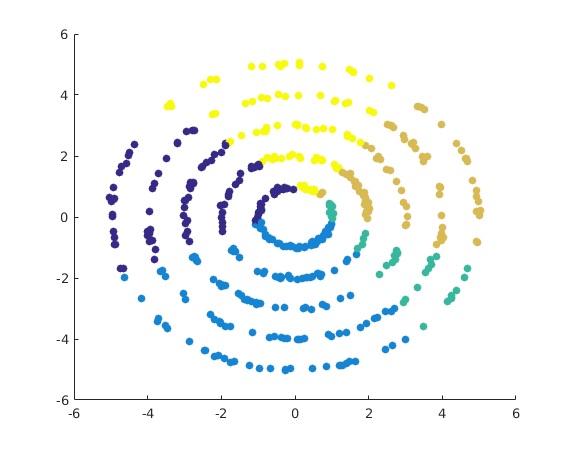
\includegraphics[width=8.5cm]{../hw2-code-data/hw2-code-data/Problem4/plot/4a_plot}
%\end{figure}
%
%\subsection{Part (b):}
%No, the results are not satisfactory, because the basic k-means algorithm assumes that the variance of the distribution of each cluster is spherical, which is not the case here (clusters are in form of rings). K-means also assumes that all the clusters have same variance which is also not true for the dataset. 
%
%\subsection{Part (c):}
%\begin{figure}[h]
%	\centering
%	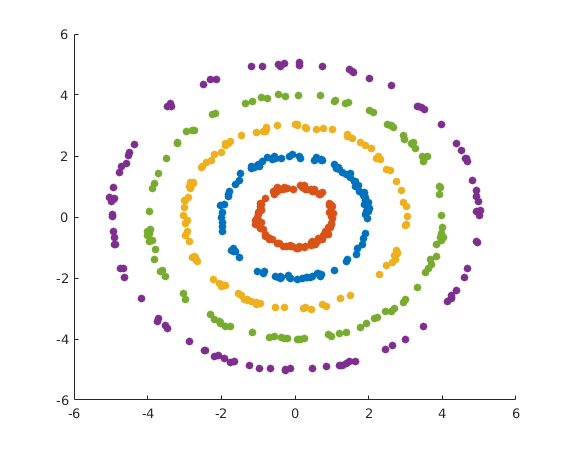
\includegraphics[width=8.5cm]{../hw2-code-data/hw2-code-data/Problem4/plot/4c_plot}
%\end{figure}
%
%\subsection{Part (d):}
%RAND score K-means: \textbf{0.6409} \\
%RAND score Kernel K-means: \textbf{1.0}
%\end{homeworkProblem}
%
%
%
%\end{document}